\documentclass[11pt]{article}
\usepackage{latexsym}
\usepackage{amsmath}
\usepackage{amssymb}
\usepackage{amsthm}
\usepackage{epsfig}
\usepackage{psfig}
\usepackage{hyperref}
%\usepackage{todonotes, listings}

\author{Oscar Moll-Thomae}
\title{Status report}

% 1-inch margins, from fullpage.sty by H.Partl, Version 2, Dec. 15, 1988.
\topmargin 0pt
\advance \topmargin by -\headheight
\advance \topmargin by -\headsep
\textheight 8.9in
\oddsidemargin 0pt
\evensidemargin \oddsidemargin
\marginparwidth 0.5in
\textwidth 6.5in

\parindent 0in
\parskip 1.5ex

\begin{document}
\maketitle


\newcommand{\code}{\ttfamily}

%todo: figure out way of placing arguments to those ops (see the if then else thing)
%todo: figure out way to make text wider
\newcommand{\edgeq}{{\code getEdge()}}
\newcommand{\fanoutq}[1][]{{\code getFanout(}~#1~{\code )}}
\newcommand{\intersectq}{{\code getIntersection()}}
\newcommand{\randomwalk}{{\code randomWalk()}}

\bibliographystyle{alpha}

\section{Background}

At Twitter, there are three main types of query operations expected of the graph store interface. One is querying for edge metadata given the two endpoints {\code getEdge(v,w)}. Metadata includes values such as a timestamp for when the edge was created, and qualifiers for edge such as whether this represents a simple 'follow', or also a  'follow via sms', or even a ''blocked'. Edges are directed, and there need not be symmetry.  A follows B does not imply B follows A, but A follows B is a fact that may be queired via both A and B. At the application level, this enables the site to inform the user  'do I follow person B?' by displaying this fact on a user's profile, or by coloring the 'Follow' button differently to indicate this is already the case.   

metadata = getEdge(vertexV, vertexW);

note getEdge(vertexV, vertexW) $\neq$ getEdge(vertexW, vertexV).


The second one is, given a vertex, return all its adjacent vertices. In a directed graph, there are two directions
to choose from. Moreover, there are variations on this, we can ask for user given number of vertices, for example the latest one, or all the   {\code getFanout(v)}, The fanout operation with a limited page size enables site visitors to look at the first few followers as well as the first few people a person follows.   Most importantly, the fanout operation enables tweet routing and delivery. Depending on the timeline materialization strategy, Whenever @LadyGaga tweets, the effects of that action must be propagated to @omoll and  everyone else following her in a way that allows for later retrieval.  Or alternatively whenver @ladyGaga signs into the service, tweets from all the people she follows can be retrieved and merged to materilize her timeline. Either of these methods, or a hybrid strategy, need of the fanout operation.


%\verb!list<Vertex>, newcursor = getFanout(vertex, inward/outward, maxResults, cursor)!

 we can scroll thorough the full intersection by either giving a large maxResults, or using the newcursor as the input for a subsequent intersection operation. The ordering of the vertices can be used to encode information, such as edge creation time or for example 'strength' of interactions etc.


Finally the third query operation is the intersection of the neighbors of two nodes: getIntersection(v,w).
There are several important use cases for this operation. When a user visits a friends page, we may want to show a limited set of common friends.  When a user visits a stranger's profile page, it may be useful to show them friends that already are following that stranger to encourage a follow.


%\verb! list<Vertex>, newcursor = getIntersection(vertexV, inwardV/outwardV, vertexW, inwardW/outwardW, maxResults, cursor)!

%%todo, flesh out examples
So, for instance we might want to intersect the the followers of @omoll with the followers of @ladyGaga.

Semantics of intersection: the result is like getting the fanouts we wish, and then intersecting them outside. Except, we know the intersection will filter out potentially many results, plus we may only need a few, so for efficiency reasons it makes sense to push the operation to the database.

The only update is to add, modify or delete an edge or its metadata. 

%note: if we order by date, we still need to  order by id because intersection depends on it.
% other compelling uses of the store could be discussed. eg naive recommendation., more complicated 

%% todo make in to table
A real workload is made of a mix of these queries and updates. Based on the query logs, the most popular type of query is the fanout/fanin query with a 

\begin{enumerate}
\item fanout(vertex, inward/outward, small, -1)  70\%. (ie, asking for the first follower)
\item fanout(vertex, inward/outward, between 1000 and 5000, -1) 10\%
\item intersection: 1.5\%
\item edges: 0.5\%
\end{enumerate}

The database also supports more complicated set operations, and these are less common.

Importantly, the maxsize given to fanout determines how heavyweight the operation is. So we can also see that
as having two lightweight operations (in terms of data returned): fanout(1) or getEdge() or heavyweight ones such as
intersection() and fanout(1000); Intuitively, these heavyweight operations need only represent 7x more work than a single light weight operation in order to be as significant in the total work done in the system as the lightweight operations.

Finally, this ranking excludes writes to edges. Which were not measured. But for every edge in the graph, there must have been a write. Also, while this work focuses on the queries, we don't visit techniques that make writing more expensive.

%%% give example for each.
The information shown about the kinds of operatons, workloads, and the kind of data stored in the grap are relevant to designing the storage system. 

This includes  areas such as the interface language (express set operations?), query processing(push operations to individual nodes?, check for wide differences in size for intersections, treat different nodes differently), data partitioning (locate followers together?) across nodes, and storage data structures (index for each view of a directed edge: from its source, or  from its destination). It also gives an idea of which things we do not need to support, such as queries about shortest paths, some version of pagerk, or general pattern matching across the whole graph. In short, the operations we have are really local operations such as counts (degree), neighbors, individual edges. Intersections are really the less local pieces of information.

\subsection{graph}
The graph has a skewed degree distribution. for both in degree and out degree.(exponent 2),  The mean indeg is at 30 or so. The max is at 1 million, 
the min is 1. The exponent matters because the larger it is, the less common the large cases are.  There is a clear correlation between in-degree and out-degree. 

%figure

%check if not 40 number.

\subsection{graph vs workload}
I explored he possibility of dependencies between the graph and the workload by checking how much degree correlated with queries.
For example, it a high degree node must have received many writes in the past. If these trends continue to the future, the perofrmance of 
queries or updates on high degree nodes is more significant than otherwise.  There was  some correlation across operations: nodes that had many 
fanout queries also were part of many intersection queries.

%%eventually place the plots in a matrix.

\subsection{my project}


\subsubsection{contributions}

\subsubsection{Two tier hashing}
The main original contribution in this thesis is the idea, that for fanoutq queries, it pays to treat heavy degree vertices different from light degree ones.  There are two factors in play here, one is,  

1) in general, the system users benefit from reducing the variance in latency across calls (which reflects an underlying variance in degree) by making it more predictable. 

2) some latencies are simply too large to be acceptable %copy back of the envelope showing this
and the problem will keep getting worse.  An important feature of a service like twitter is the real-time feel it gives its users. It is undesirable to  becomes notable that some users receive tweets much before others. This also implies more complicated design within the rest of the system, as application logic demands no user sees a reply to a tweet before receving the tweet first.  Hence, extra work is done at different layers to hold on to tweets that cannot be delivered yet, 

This property is present in many naturally arising relations. eg. social networks etc.

This feature comes at the cost of complexity in the sharding mechanism. In fact, since there is no relation between the user id and whether it has a large degree, it is necessary to introduce lookup tables for this purpose. Luckily, we can use the graph property that  the degree is very skewed against itself: we only need to remember very few. 

%todo add another back of the envelope

This condition is helpful it would not be less plausible with a graph where there are two equally large classes of nodes to have a table for half those cases. in that case, though, we can do something such as cacheing, in case access patterns show some kind of skew. %complexity problems related to look

%(actually it would be interesting to analyze how cacheing relates to this, and maybe propose a solution based on it. Cacheing depends on skewedness in access patterns (ie acesess are only like to a few places), but cacheing policies can normally adapt online to handle distributions that change over time, as long as they remain skewed.

For a given fanout size, there is an optimal number of partitions with respect to latency. For throughput, the optimal is probably  closer to 1.

The two main factors potentially afecting latency are 1) variability in network communication: the more nodes we request data from, the more likely
at least one will lag, affecting the performance of the whole operation 2) the more nodes we have, the more parallelism there is in reading.

These factors can be expressed as \(L = max_{i=1}^n(L_i) + q*d/n\), \(q\) is a system specific constant, \(d\) stands for a fixed degree, so we are splitting the fanout into many and the latencies \(L_i\) are random, with some distribution (eg exponential). Presumably the \(f(n) = E[max_{i=1}^n(L_i)]\)  is an increasing function of \(n\). so \(E[L]  = E[max_{i=1}^n(L_i)] + work/n\). DeWitt etal  model this by  assuming \(L = kn\) for some system specific constant \(k\).  With that assumption, optimizing \(n\) to minimize latency is straightforward.

The above analysis was valid for a particular \(d\) variable. So this would be the optimal partitioning for vertices of a particular degree.  Where there is variation of degrees, in the best possible world we would treat each node according to its degree. A sharding function would need to figure out based on the node how to treat it, so we would need a lookup table for that. This would be unrealistic (right?). unless we keep a table of size O(number of nodes).

Alternatively, it is feasible to degrade the granularity, and pick a threshold \(B\) such that we  divide all nodes with \(deg > B\) one way, and the rest another.

Given a B, We can optimize differently for each part (and also, we can further optimize for the B) and implement this by remembering only the nodes above the threshold. This way we get a much smaller lookup table.  Optimizing for each of these independently brings together many strategies that may seem very different if treated in isolation (such as shard everyone into 2 parts no matter the degree,  or  for degrees above 10k,  shard into all machines) and picks the best.

(this more careful analysis still needs to be done)

Potential problems are how the optimal changes as the graph grows.

%todo. Analysis of added problems of sharding mechanism in dynamic situation.

\subsection{experiments}

Designed a benchmark with skew on ID queried, but iid. Designed a way of generating graphs for querying fanouts (random degree). The benchmark allows me to control 
query skew, while the graph allows me to control degree skew, or a constant degree.

The argument about skewed degrees and lookup tables implies that the more skewed a degree is, the easier it is to implement lookup tables. while also the less relevant it is
(because having only 1 large user and 1 million small ones means it might be acceptable to degrade. On the other hand, if skew is 1, then actually 'work' graph is very uniform.and if the parameter is less than 1, the work is actually all concentrated at the top!, so arguably you should design for it.

ie. let  \(D\) be the random variable representing the degree of a randomly picked vertex. Assume \(D\) has a distribution \(p_D(n) 1/n^\alpha \) then let \(E \) be the degree of an edge, where we define the degree of an edge to be the number of other edges in the same node. (directed? or sum?). \(p_D \) and  \(p_E \) are related in the following way:

\( p_E(n) = n*p_D(n)\). This relation expresses that in a graph with vertices of varied degree, edges are more likely to be around large degree nodes. 



 is making cases where \(n \) is large more likely. 

Caveat: cacheing and size control. How can we 1) increase the degree of every node 2) keep total database size constant 3) not increase locality.
I gave up on keeping database size constant, so some database were more full than others. To avoid cache effects. (not even sure if i controlled this effect well)

Note on experiments:
The two tier version is not great because while I had seen for 5 nodes partitioning into 3 parts is best, this was not the case i nthe benchmark.
In fact, partitioning everyone seemed to be the best choice.



\subsubsection{real data and workload}
I experimented with a snapshot of the Twitter graph and three different strategies. The first is the control:  hashing by vertex, 
The second is the two tier strategy, and the third is the workload based partitioning approach.

\subsubsection{control}


\subsubsection{two-tier}
Ran it with a threshold at ??(top 1m) into 5 parts.  Latency behaved as follows:


The bad news are I arrived at this setting through tuning a program that was not well optimized, after I optimized it.

%% \begin{figure}[h]
%%   \begin{center}
%%       \scalebox{1}{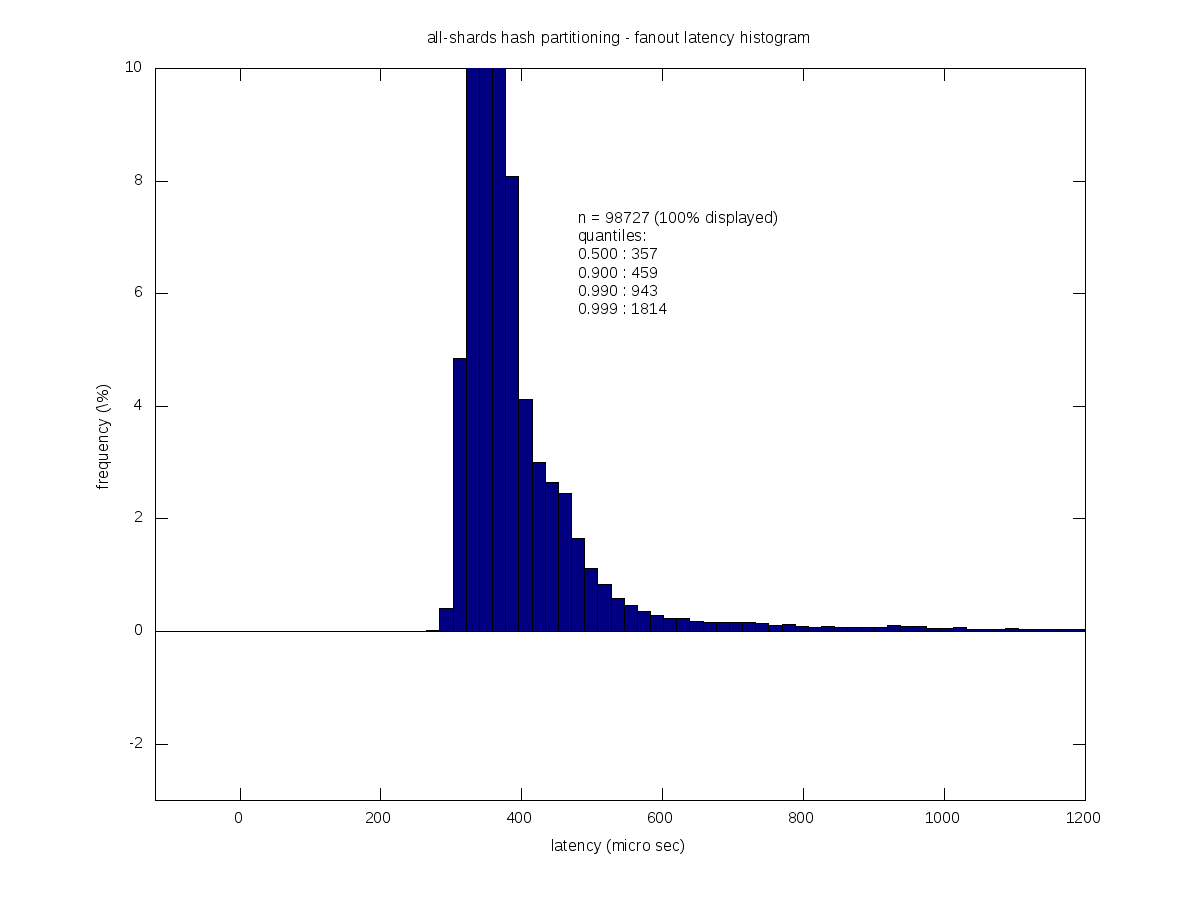
\includegraphics[width=6in]{all-shards-fanout.png}}
%%   \end{center}
%%   \label{all-shards-fanout}
%%   \caption{\small Results for all-shards strategy.}
%% \end{figure}


So when I checked to see performance for 5 way partitioning everything, I got evenmore improvements for the higher latency ranges.

\subsubsection{workload}
Not sure of re



\section{Design}
%information about what I built, (java and pig) goes here. information about results goes here too.

To test the different strategies I constructed a basic system consisting of query router server and  several data notes in the backend.  The query backend server 

%diagram goes here
\end{document}
